\section{Evaluation} \label{section:evaluation}
We conducted a user study to compare \tool to a \baseline tool. \baseline only contains the features present in current property booking tools (e.g. Airbnb \cite{airbnb} or Booking.com \cite{booking}) and collaborative search tools (e.g. SearchTogether \cite{searchtogether} or ResultsSpace \cite{resultsspace}). It contains a search page along with the \collabQueryPanel, a chat, and a bookmarks page that shows a list of bookmarked properties. The bookmarks page is similar to Airbnb's wishlists or the summary section of SearchTogether~\cite{searchtogether}.  \baseline has a similar UI aesthetic to \tool.  

The goal of our study is to  (i) assess if users of \tool can reach more satisfying agreements when compared to \baseline, (ii) determine if there are differences across both tools in how and when users conduct the different tasks (Section \ref{ssection:task}) associated with group booking, (iii) qualitatively evaluate the utility of \tool's novel features in the context of the challenges we identified in Section \ref{ssection:challenges}. 

\subsection{Methodology} \label{ssection:methodology}
Twenty-one participants were recruited to use \tool, and twenty-one were recruited to use \baseline. User study participants were recruited from a university's academic and residential mailing lists. The lists' subscribers included former and current university employees (staff and faculty), alumni and students, as well as non-university affiliates who resided on campus. Participants recruited  were between the ages of 18 and 37, 50.0\% identified as female and 50.0\% as male.  85.7\% have a high school diploma and 14.3\% have a college degree or higher. Of those with a college degree, 57.1\% had a degree in STEM (Science, Technology, Engineering, and Mathematics), 28.6\% in Social Sciences, 14.3\% in Arts \& Humanities. 69.0\% reported having experience collaborating with people over the web. 

Participants took part in a zoom session where they received a tutorial on \tool or \baseline. Participants were encouraged to ask clarifying questions at all times during the tutorial session to ensure proficiency with the tool. In addition, participants had access to video tutorials prepared by the researchers. Any emailed questions were answered at the researchers' earliest convenience throughout the duration of the multiple-day study. 

Participants were asked to complete a pre-experiment questionnaire where they signed a consent form and reported simple biographical information (i.e. age, gender, and education) and their experience with search and digital collaboration. 

To ensure the participants are committed to the task at hand, a commitment akin to that of an enthusiastic tenant-to-be rigorously searching as they are to make a substantial time and financial investment, participants were tasked with being the personal-shopper of an avatar that has specific requirements for their home. The avatars' descriptions are attached in Appendix \ref{appendix:avatars}. The participants were then placed in a random anonymous group of 3 participants, each representing an avatar. The participant in the group that best represented their avatar's requirements in the final selected property received a monetary bonus. We acknowledge that the participants in this study do not elicit the same sense of personal investment as the avatars they represent would in real life. The avatar user study provides a controlled environment that allowed us to accommodate a variety of testing conditions particular to \tool. More specifically, it allowed us to study the effects of conflicting preferences in group dynamics and decision-making (e.g. smoking vs not-smoking or conflicting budgetary constraints as seen in Appendix \ref{appendix:avatars}). It gave us flexibility in recruiting participants and pairing them in groups with ease and at scale. Finally, the monetary reward gave participants a motivating drive to push for their avatar's interests within the group. 

Participants were told to look for a property in New York City for a week-long vacation using \tool. \tool's database was populated with properties from New York City to resemble as close as possible a real-life scenario. 

Participants participated in the study asynchronously and remotely for up to 5 days. Participants were asked to log in periodically to the tool and search with their team members. No form of micro-management or timing requirements were imposed. The anonymity of the participants ensured that the tool itself was the only communication medium amongst the team members. 

Users using \tool were asked to come to an agreement by all of them signing a contract. Users using \baseline were asked to send a screenshot of the final agreed upon property via email to the researchers as the tool did not possess an embedded agreement system. 

After concluding the study, participants were asked to complete a post-experiment questionnaire where they rated the tools they used and the features contained wherein. After the participants completed the questionnaire, their participation payment and any earned bonuses were processed. 

This study received approval from the Institutional Review Board (IRB) under the Exempt category. Participants were compensated with 14 USD for their participation in this study. Furthermore, within each team, the participant whose avatar's preferences for their dream home were satisfied the most was awarded a bonus of 27 USD. 


\subsection{Results} \label{ssection:results}
We begin by stating that our results must be taken with a grain of salt: Our positive results are simply promising indications that \tool's design does support collaborative property search and agreement. Our surfaced patterns and observations are exciting, but merit future confirmatory research. Our study size is relatively small though not unusual for HCI studies of this nature (e.g. 14 participants for SearchTogether \cite{searchtogether} and 14 participants for ResultsSpace  \cite{TeamSearch}). Please refer to Table \ref{tab:lit-comparison} for a more comprehensive comparison between \tool and previous work. 
Small study size is due to the challenges involved in recruiting and managing participants for a collaborative, effort- and time-intensive, multi-day study. 
We present our results not with the expectation that they can immediately generalize to how users will actually use a tool like \tool in the wild (Section \ref{ssection:studylimitation} describes some of the study design limitations and justifications); rather our goal is to illustrate how \tool's design influenced the complex behavior and  dynamics of teams of users as they interacted with \tool asynchronously over multiple days when compared with a \baseline that mimics the state of the art in collbarative search. We hope our results motivate researchers to consider designing collaborative search and agreement tools using our design principles and further study the impact of some of our proposed features.
%}

\subsubsection{Can users of \tool reach more satisfying agreements when compared to \baseline?}

\begin{itemize}
    \item All seven groups with three participants each using \tool  signed a contract.
    \item Six of the seven groups of three using \baseline were able to agree on a property within the study.
\end{itemize}

Based on a 5-point Likert scale question that asked users to rate their overall degree of satisfaction with the property chosen by the group in the post-study questionnaire,
\begin{itemize}
    \item The average rating across users using \tool was 4.52 ($\sigma = 0.68$ \fiveBucketsHistogram{0.000}{0.000}{0.095}{0.286}{0.619}).
    \item The average rating across users using \baseline was 4.00 ($\sigma = 0.98$ \fiveBucketsHistogram{0.000}{0.083}{0.208}{0.333}{0.375}).
\end{itemize}
    
In examining the impact of the tool used on the degree of satisfaction, a linear mixed-effects model was employed to account for the nested structure of the data due to the teams the users were grouped in. The fixed effect of using \tool, as opposed to the reference \baseline tool, was found to be marginally ($\alpha = 0.10$) statistically significant ($\beta = 0.429, SE = 0.257, z = 1.670, p = 0.095$). This suggests that using \tool is associated with a marginally significant increase of approximately 0.429 units on the 5-point Likert satisfaction scale. Additionally, the variance attributed to the random effects of the teams was negligible, indicating minimal variability ($\sigma^2 = 0.000, SE=0.151$) in tool satisfaction due to team assignment\footnote{We note that the Q-Q plot of residuals closely follows the 45-degree reference line with slight deviations in the tail, suggesting residuals are approximately normally distributed. It is challenging to discern any patterns in the residuals vs. fitted values plot due to the limited number of data points. The Variance Inflation Factor (VIF) assessment for the predictor \tool yields a value of 1.0, indicating no multicollinearity concerns. Thus, the diagnostic plots do not present strong violations to the assumptions of the linear mixed-effects model, but the limited number of data points necessitates a more cautious interpretation of the model's assumptions.}. 

In \tool, the average number of satisfied requirements per user was 2.7 out of a maximum of 4 possible requirements ($\sigma = 0.54$) and in the \baseline it was 2 satisfied requirements per user ($\sigma = 1.01$). A requirement is satisfied if the property explicitly satisfies it (e.g. the amount paid by a user is within their budget, the property has a kitchen and the user wanted one), or if an explicit workaround is agreed upon either through chat messages in \baseline or contract house rules in \tool (e.g. getting a property with a sound system but agreeing on quiet hours to satisfy users that enjoy loud music and users that appreciate quiet nights). We again conducted a linear mixed-effects regression analysis to account for the random effects of team assignment. The fixed effect of using \tool as opposed to the reference \baseline tool --- an increase of 0.667 satisfied user requirements --- was found to be marginally ($\alpha = 0.10$) statistically significant ($\beta = 0.667, SE = 0.404, z = 1.650, p = 0.099$).  

This improvement is appreciable as there are only four requirements per user overall and at least two requirements may conflict with the requirements of other users within a team\footnote{The diagnostic plots do not show strong violations of the assumptions of a linear mixed-effects model.}. As expected, the variance attributed ($\sigma^2 = 0.397, SE = 0.365$) to the random effects of team assignment is considerable. This makes sense: e.g. teams that do not agree on a property will have zero satisfied requirements for all their members. 


\subsubsection{Are there differences in how and when users conduct tasks across the tools?\\}

\begin{figure}[htb]
    \centering
    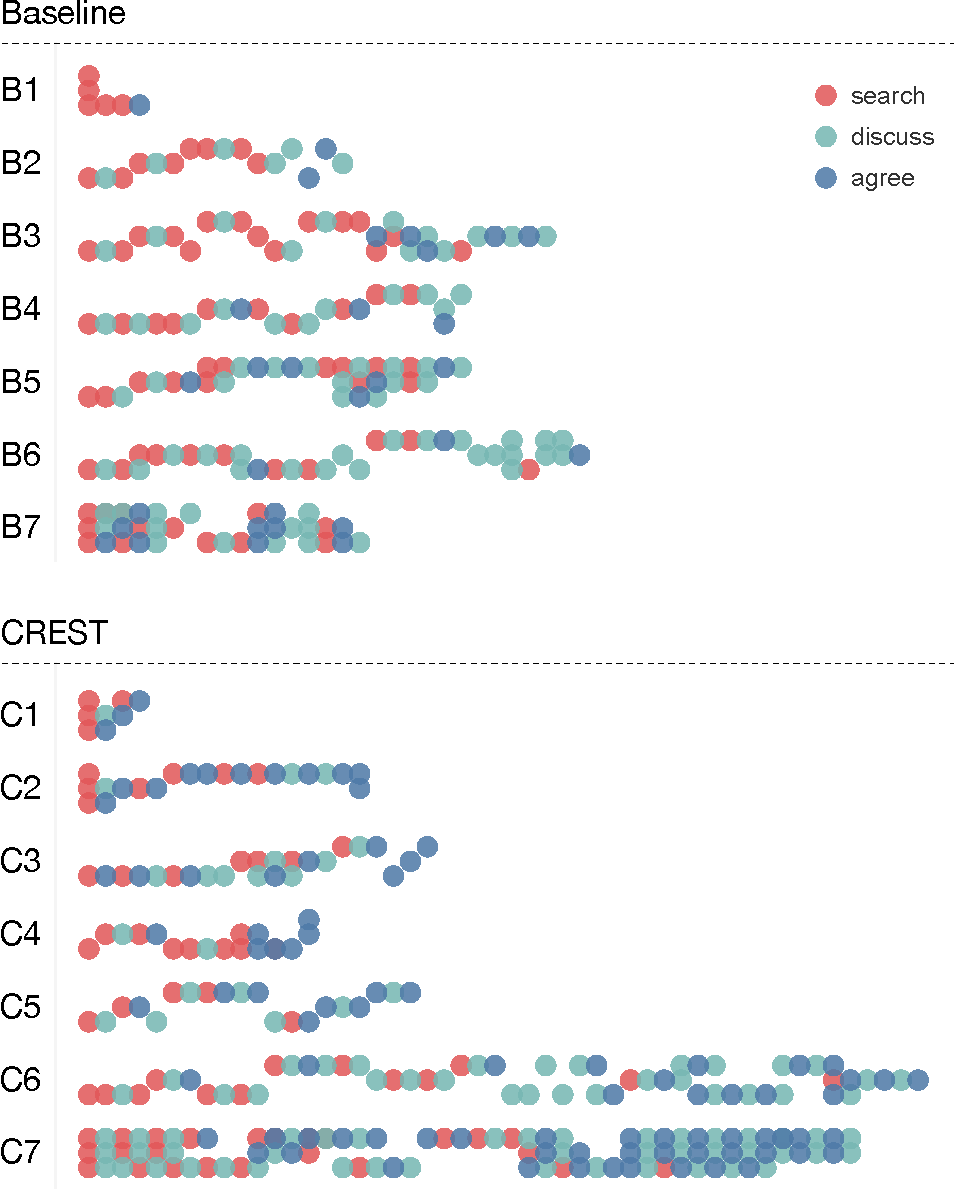
\includegraphics[width=0.6\linewidth]{images/logical-timelines.pdf}
    \caption{An overview of the sequence of events that occurred in each group across its three users. Users are ordered vertically. Events are logically ordered along the horizontal order axis. A single event captures one or more consecutive actions of a task type (search, discuss or agree) that occured within a user's session. In situations where users were active during the same time span, their events might have the same logical order. We opt for logical order instead of physical timestamps due to the asynchronous, multi-day nature of the study: users were disconnected for large time periods with infrequent bursts of activity. B6 is the only group that failed to agree on a property to book.}
    \label{fig:timelines}
\end{figure}

\smallskip To understand differences in user behaviour across both tools, we instrumented them to track as many activities as possible on the user interface. These activities included log-ins, clicking on any button or link or sending a chat message. Certain activities could not be tracked e.g how long each user dwelled on search results or scrolled through them, or if/when they logged-out. This tracking is facilitated by \tool's system architecture described in Figure \ref{fig:crest-architecture}. Not only do we save every single user action that occurs within \tool in our database as a byproduct of implementing a full-stack tool, but we also implement a dedicated logging service that tracks all major events (i.e. "User 1 added preference refrigerator in Team 2") in a table in our database.

We then grouped each of these tracked activities into the three main actions involved in group booking: search, discuss and agree. \textit{Search} included activities like adding, modifying, liking or disliking a user preference, clicking on a property for more details, bookmarking it, etc. Two of the authors conducted a natural language analysis of the messages to classify them into the two remaining categories: \textit{Discuss} and \textit{Agree}. Both authors used a simple heurestic to aid this labeling: if a message mentioned a specific property, it was most likely seeking agreement on it and was often labeled `agree', other messages were often labeled `discuss.'



Figure \ref{fig:timelines} illustrates how the collaborative booking progessed within each of 14 teams. We note the asynchronous nature of the study with users often being active at different times. 

We provide the figure for reference noting that it is difficult to infer general patterns from fine-granularity sequences. However, we can observe that most sequences begin with users alternating between search and discussion tasks and then conclude with users alternating between discussion and agreement tasks. We find users engaging in more agreement activities with \tool than in the \baseline. B6 is the only group that failed to book a specific property at the end of the study.

We observe that groups using \tool engage in agreement activities earlier than in \baseline. To better visualize this phenonema, we normalized all event sequences on a scale of 0-100 and then for each group plotted when the first agreement event occurred as follows:\\[0.1cm]
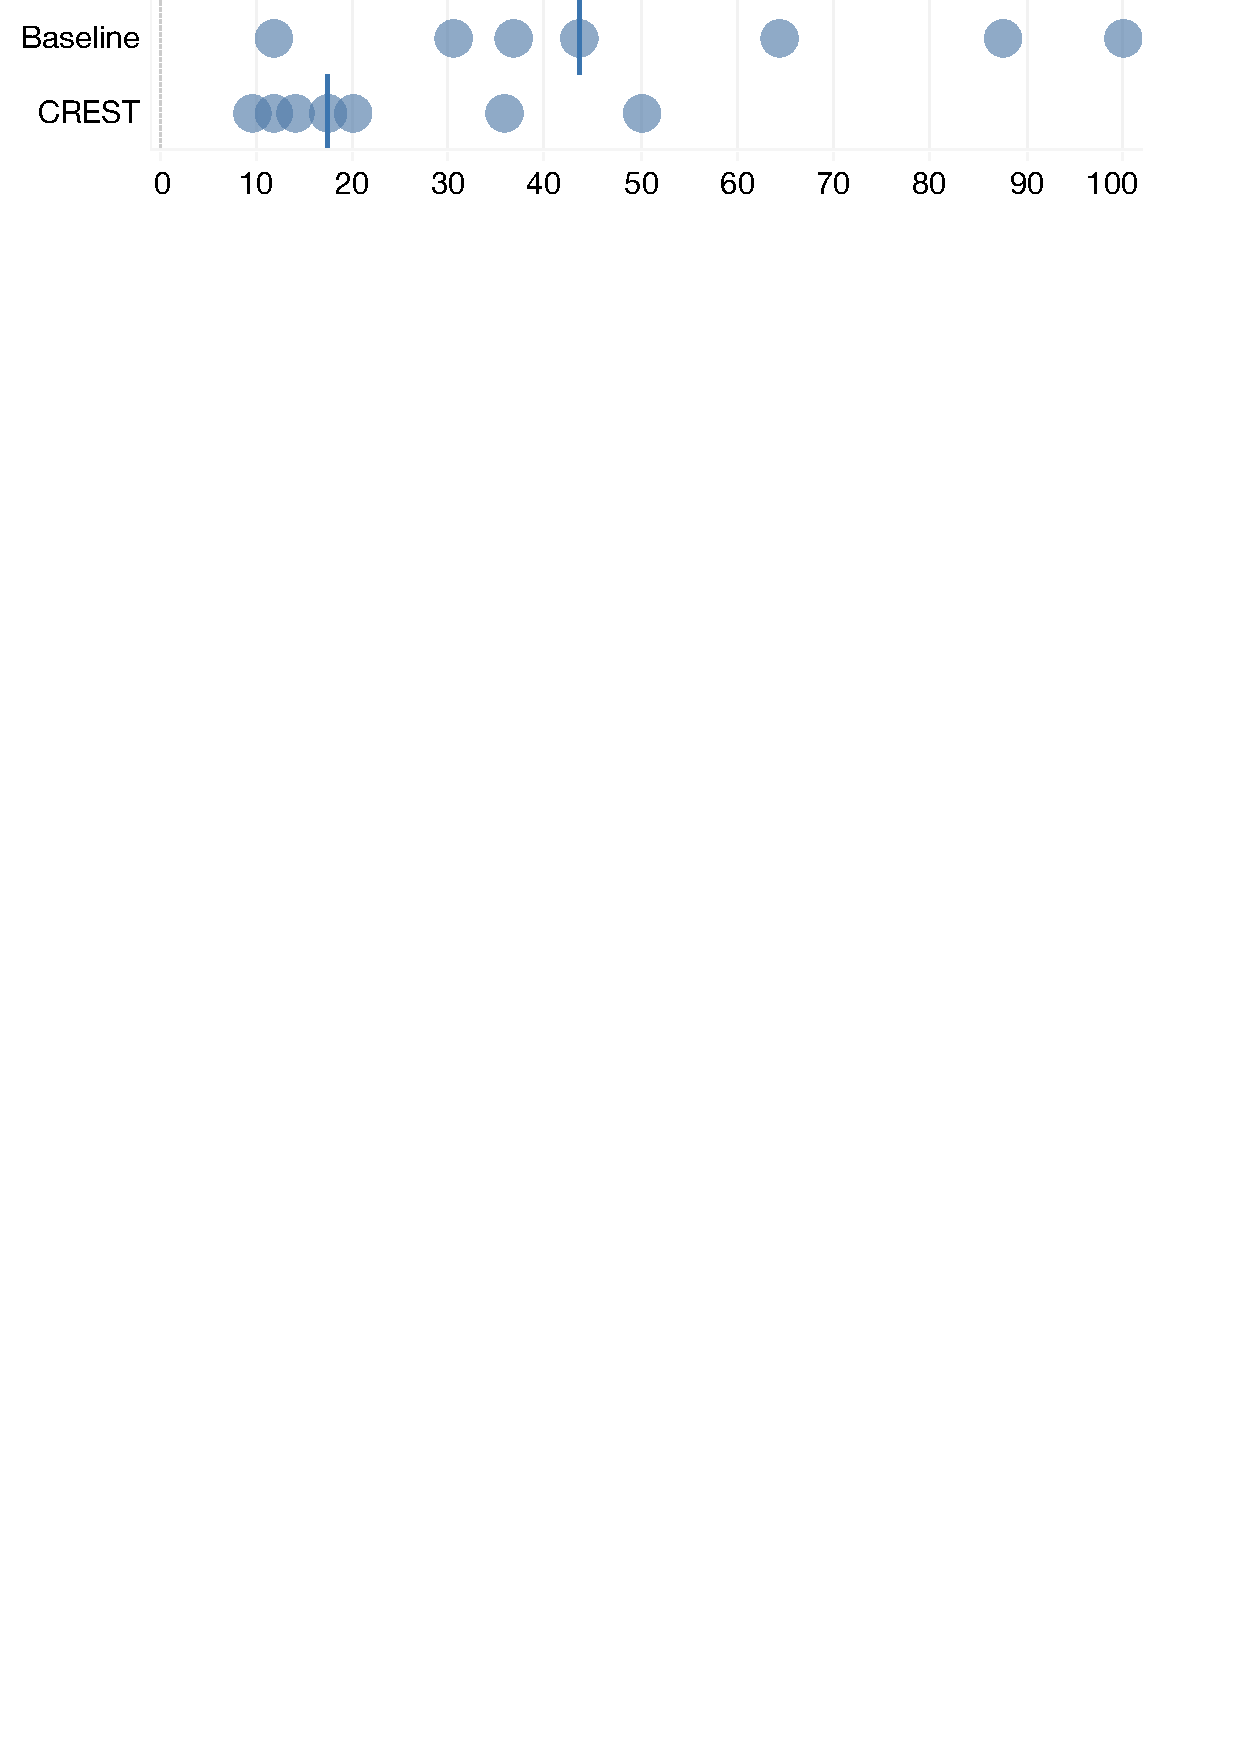
\includegraphics[width=300px]{images/Agree.pdf}\\[0.1cm]
A one-way analysis of variance (ANOVA) shows a statistically significant ($\alpha = 0.05$) difference in the means of the first agreement event across the tools ($F_{1, 12} = 5.33, p = 0.0396$)\footnote{We caution readers on the statistical interpretation of this result as there are only seven observations per group, which were the result of some data transformation and aggregation.}.


This possibly alludes to the efficacy of \tool's goal-centered design at driving group members towards collaborative agreement. 


Similary, we plotted the last search event for each group. \\[0.2cm]
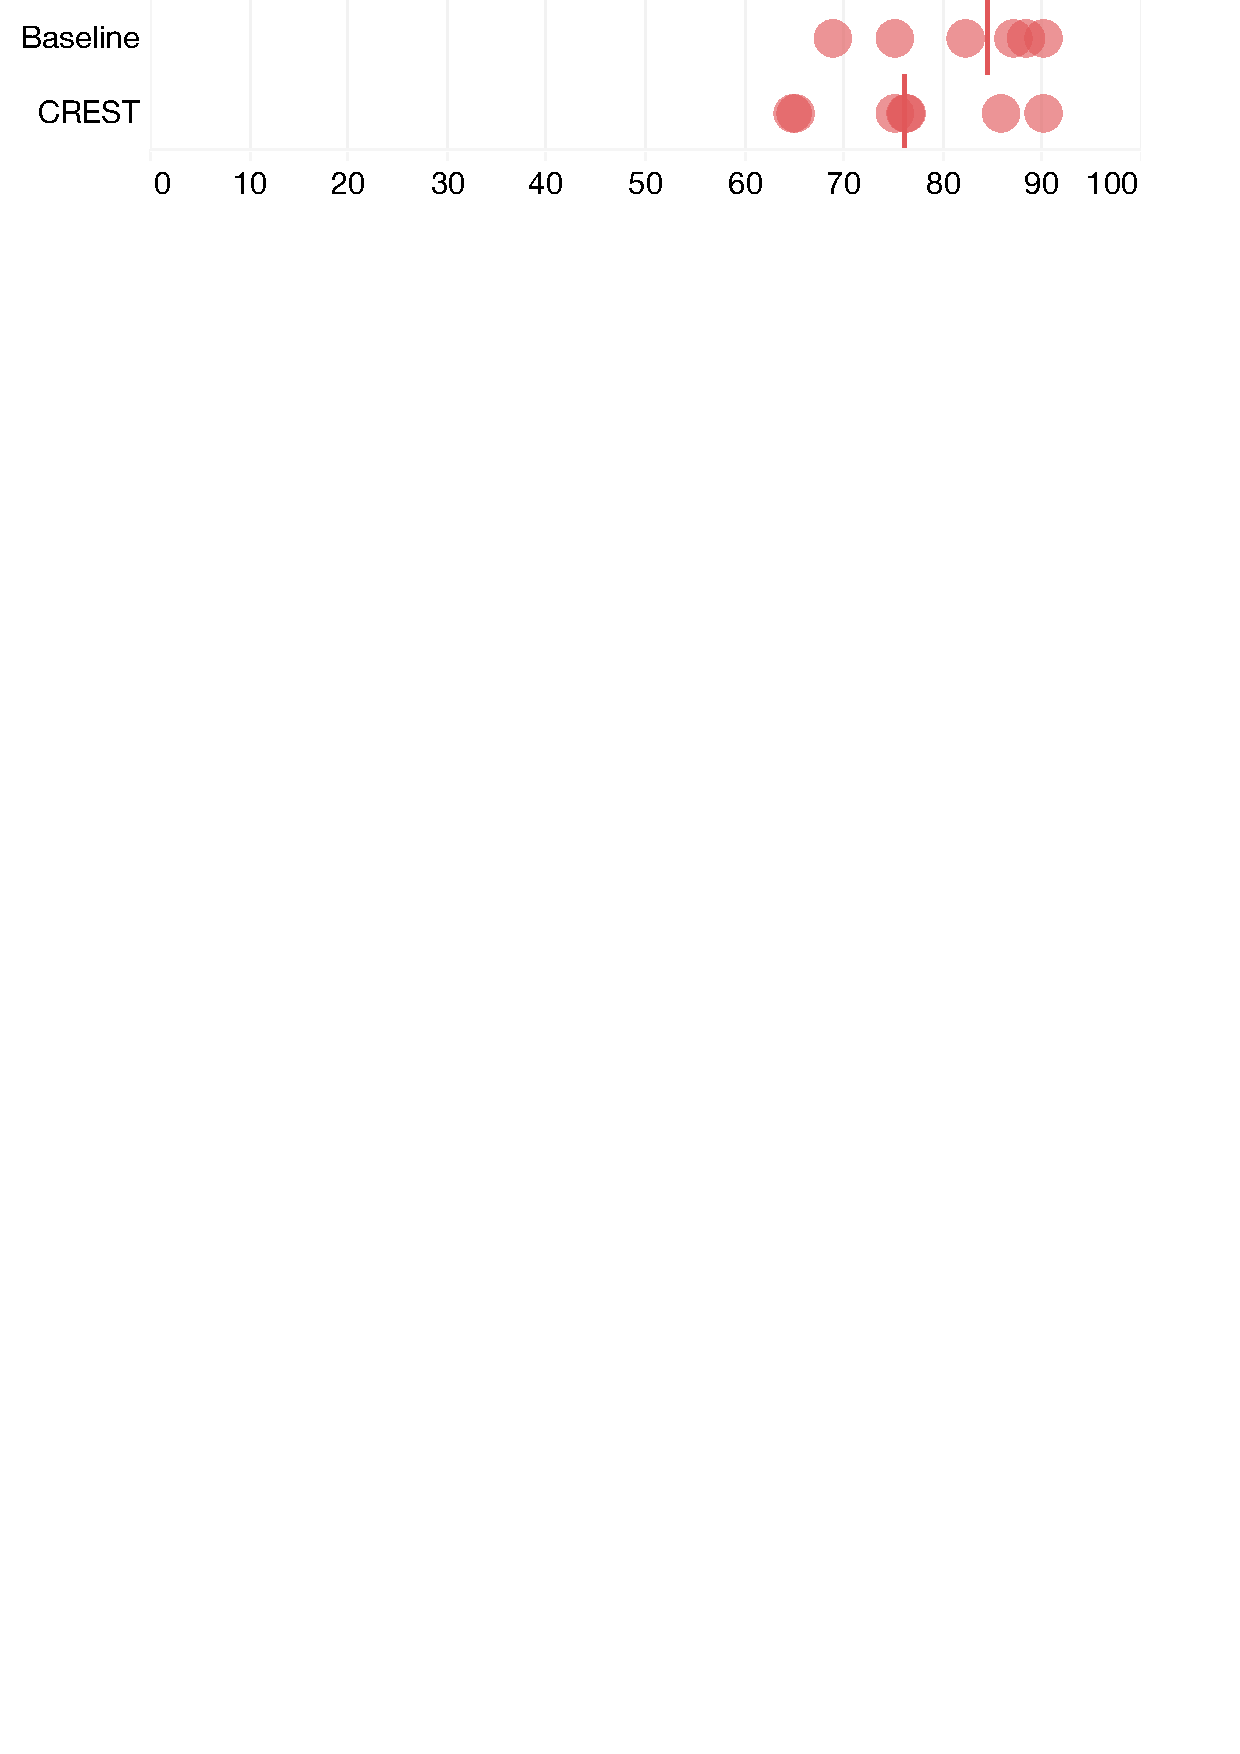
\includegraphics[width=300px]{images/Search.pdf}\\


We find some indication of a slightly more extended search with the \baseline tool hinting at the shifting goal posts challenge, however, the differences are not statistically significant (one-way ANOVA: $F_{1, 12} = 1.919, p = 0.191$).

We also find that engaging in agreement activities earlier in \tool does not limit exploration. On average, \baseline teams created 7.0 ($\sigma = 1.83$ 
) bookmarks  and \tool teams created 6.43 ($\sigma = 3.05$ 
) contracts.

 We conducted a linear mixed-effects regression analysis to determine if there are any differences between how many contracts or bookmarks are created per user accounting for variablity due to team assignment. The results suggest that with the \baseline tool, users bookmark on average 2.333 properties $(SE = 0.393, z = 5.943, p < 0.001)$. Users create slightly less contracts with \tool $(\beta = -0.190, SE=0.555, z = -0.343, p=0.73)$, but this difference is not statistically significant\footnote{In addition to evaluating the effect of version differences, our linear mixed-effects model also accounted for variability introduced by the distinct teams. We identified a sub-group variance of 0.007. This suggests that while there exists some variation in bookmarks or contract counts across the different teams, it is relatively small. As with our previous mixed-effects analysis, we find that the assumptions of linearity, homoscedasticity, independence, and normality are satisfactorily met.}. 
 
 Compared to proposing contracts, bookmarking a property is a simpler action to perform when openly searching for viable options. This is because proposing contracts immediately frames users into thinking of the team as a whole, the house rules to propose, and all the intricacies of team decision-making required by this feature. Despite the higher mental toll required by \tool, users of both tools collected and considered a similar number of high-quality properties. \tool teams, however, had the added advantage of engaging in more agreement-specific activities as explained in Section \ref{sssection:novel-features} with each property they considered. 

 Moreover, even though a similar number of contracts and bookmarks are created, the challenge of shifting goal posts is not as pronounced in \tool as each contract presents a property along with the user agreements that would apply if chosen by the team. Thus, users are possibly introducing new properties only after fully considering past ones and finding them less desirable for themselves or the group.
 

\subsubsection{What are the reported user experiences with \tool's novel features?}
\label{sssection:novel-features}

\paragraph{Contracts \& House Rules as implementations of \tool's Three Design Principles}
We asked \tool users to elaborate on their experiences with contracts and house rules. Users gave an average rating of 4.45 ($\sigma = 0.6$ \fiveBucketsHistogram{0.000}{0.000}{0.048}{0.429}{0.476}) when asked to rate how helpful \tool's contracts were in facilitating group collaboration.
One user's comment alludes to how contracts achieved a goal-centered flow for them: 
\begin{quote}
``\textit{Signing a contract helped our group to be more organized in terms of decision-making. If one member was happy with several properties, he/she can sign under the property and others can decide whether to sign or not after. It is an easier way of seeing the person’s choice which then leads to adjusting to it accordingly or signing another contract.}"
\end{quote}
The comment also reveals how this user saw signing as a way of giving users individual decision-making autonomy and a contract as a space where users are made \textit{aware} of others' choices.

Another user noted:
\begin{quote}
``\textit{It was one of the key components on allowing us to stand for the same property. Regarding
smoking, we had a different opinion, but through the House rule features, we could find common ground.}"
\end{quote}
Given the conflicting nature of this team’s disagreement (smoking vs no smoking), it is promising to see that
the house rules can be used as a space to ideate solutions to otherwise difficult-to-resolve conflicts. Specifically, 4 out of the 7 contract teams addressed the smoking vs. not-smoking conflict using the house rules feature. From the teams that didn't, we failed to see in the message logs any attempt to solve this conflict in writing, meaning that this conflict remained unresolved. This phenomenon is also present in the \baseline teams, further accentuated by the lack of a conflict-resolution mechanism.

We also asked \baseline users to elaborate on their agreement experiences. We find users surfacing challenges due to conflicts and statemates and discontinuity in their comments:
\begin{quote}
\textbf{\textit{Conflicts and Stalemates:}} ``\textit{We didn’t reach an agreement. I was adamant with the Art filled apartment but the other one wanted
this luxury apartment. Maybe needed more time?}" 
\end{quote}
\begin{quote}
\textbf{\textit{Discontinuity:}} ``\textit{[Agreement] was highly dependent on the others being responsive which I
guess because of personal schedules that weren’t the case.}"
\end{quote}

We also wanted to understand why the average satisfaction with the selected properties among the two groups that reached agreement in \baseline was lower than with \tool. We found that in one of the two groups, a single user dominated the task and got what they wanted (hence reporting a score of 5 in terms of satisfaction) while ignoring the needs and wants of the other group members, who reported much lower satisfaction scores (2 and 3). The lack of decision-making autonomy and the absence of mediation strategies beyond chat-based discussions might have led to discontent within this \baseline group.

\paragraph{\cbot as \citeauthor{themediationprocess}'s ideal mediator}
We asked \tool's users to rate on a 5-point Likert scale how helpful they found \cbot's notifications and messages in supporting their collaborative task and with conflict resolution. The average rating was 4.1 ($\sigma = 1.07$ 
\fiveBucketsHistogram{0.048}{0.000}{0.190}{0.286}{0.429}).%
We also asked users to elaborate on their ratings. We find the user comments to surface some of the mediation roles (Table \ref{tab:messages}) that we designed \cbot's messages around. 
\begin{quote}
\textbf{\textit{Facilitator:}} ``[The messages] were encouraging, welcoming, and informative."  
\end{quote}
\begin{quote}
\textbf{\textit{Communication Opener:}} ``It periodically reminded us if anyone was quiet for long"  
\end{quote}
\begin{quote}
    \textbf{\textit{Leader}}: ``If it wasn't for the bot I would have forgotten to use the app, definitely the most useful part"
\end{quote}
\begin{quote}
  \textbf{\textit{Agent of Reality: }} ``Good prompts and suggestions."
\end{quote}
\begin{quote}
\textbf{\textit{Trainer, Legitimizer: }} ``It was nice how it taught me to tag someone in that chat to push them into talking about their interests."
\end{quote}

We also analyzed how often users engaged with \cbot's messages and notifications: \textit{were they largely ignored?} This analysis is possible as all messages have action buttons, such as \button{propose a contract} or \button{see property}

(See Section \ref{ssection:principles}). We tracked how often the action buttons were clicked. Here, again, we group notifications and messages into three action categories: 

\begin{enumerate}
    \item Search: These are the notifications that appear on the search page and usually expand resources by encouraging users to see a property or propose a new contract.
    Across all groups, there were 743 such notifications shown and 143 were clicked (19.25\% click rate).
    
    \vspace{0.1cm}
\includegraphics[height=10px]{images/clicks/search-with-label.pdf}
    
    \item Discuss: These messages appear in the chat and usually legitimize the rights of other members by encouraging, for example, most active members to engage the least active ones. Across all groups, there were 26 such messages, 8 were clicked (30.77\% click rate).

    \vspace{0.1cm}
\includegraphics[height=10px]{images/clicks/discuss-with-label.pdf}
    
    \item Agree: These are the notifications that appear on the contract page and usually train users in negotiation by suggesting the creation of house rules or the redistribution of monetary contributions, act as agents of reality by pointing out difficulties in finding better alternatives, and move the process forward by encouraging negotiation or contract signing. Across all groups, there were 2 such notifications, 1 was clicked (47.9\% click rate).

    \vspace{0.1cm}
\includegraphics[height=10px]{images/clicks/agree-with-label.pdf}
\end{enumerate}

We find that \cbot's messages and notifications are not ignored, especially those that move agreement along or empower users to negotiate better. The low click rate on search notifications is not unusual: these notifications act as property recommendations, and users may disagree with the recommendations or may already be content with the existing pool of properties/contracts under consideration. 

We further classified each message generated by \cbot into one of the seven mediator roles it impersonates (See Table \ref{tab:messages}). We find messages that challenge users with difficult preferences (Agent of Reality) and those that provide mechanisms or suggestions to promote negotiate (Facilitor/Trainer) are more likely to be clicked than other messages (See Table \ref{tab:clickratio_by_role}). Further studies, however, are needed to better determine the effect of \cbot's mediator role on user engagement.
\begin{table}[]
\resizebox{0.48\textwidth}{!}{
\begin{tabular}{lp{0.40\linewidth}c}
\toprule
\textbf{Role} & \textbf{Click-ratio} & \textbf{Messages} \\ \midrule
Problem explorer & \PercBar{0.17}{2.6cm} & 566 \\

Legitimizer & \PercBar{0.19}{2.6cm} & 472 \\
Resource expander & \PercBar{0.19}{2.6cm} & 617 \\

Leader & \PercBar{0.30}{2.6cm} & 289 \\
Comm. opener & \PercBar{0.31}{2.6cm} & 26 \\

Facilitator \& Trainer & \PercBar{0.34}{2.6cm} & 38 \\

Agent of reality & \PercBar{0.34}{2.6cm} & 145 \\
\bottomrule
\end{tabular}
} 
\vspace{0.2cm}
\caption{How often users clicked a message reflecting one of \cbot's mediation roles. A message can belong to multiple roles (See Table \ref{tab:messages}).
}
\label{tab:clickratio_by_role}
\end{table}



\paragraph{\tool's Awareness-guided features}

Users commented on their experience with \tool's visualizations and different components such as the \collabQueryPanel that shared the current state of search preferences for the entire group. We find that the visualizations not only helped mitigate discontinuity challenges but it also motivated participants to move the task forward and positively engage in the process.
\begin{quote}
\textbf{\textit{\collaboRatio:}} ``\textit{The activity / influence / communication graph is great at illustrating who has more say in the decision-making which is very interesting. The team’s preferences were also well-illustrated in icons which I personally found very easy to navigate}'' 

``\textit{from the visualization [it ] seems I
was the least active in the group, so I just followed the group suggestions more}''

``\textit{It gave everyone a personal responsibility to stay active and collaborate}''
\end{quote}

\begin{quote}
\textbf{\textit{\collabQueryPanel:}} ``\textit{I find that interests are best communicated through the shared filters}'' 
\end{quote}


Finally, we asked the users to report on a 5-point Likert scale how easy completing a group booking exercise was on \tool or \baseline. We also asked the users who used tools like Airbnb or Booking.com how easy it would be for them to collaboratively book a property with these tools. The mean ease-of-use ratings of \tool, \baseline are respectively $4.24$ ($\sigma = 0.89 \fiveBucketsHistogram{0.000}{0.048}{0.143}{0.333}{0.476}$) and $3.92$ ($\sigma = 0.78
\fiveBucketsHistogram{0.000}{0.042}{0.208}{0.542}{0.208}$). 


In examining the impact of the tool used on user-reported ease of use, we used a linear mixed-effects model to account for the participants working in teams\footnote{We find that the assumptions of linearity, homoscedasticity, independence, and
normality are satisfactorily met.}. The fixed effect of the tool on ease-of-use ratings was statistically ($\alpha=0.05$) significant ($\beta = 0.571, SE = 0.288, z = 1.984, p = 0.047$). Using CREST is associated with a  significant increase of
approximately 0.571 units on the 5-point Likert ease-of-use scale even when accounting for variations from team assignment. The random effect,

 which captures variability due to team assignment, also had a significant contribution to the model ($\sigma^2=0.171, SE = 0.225$).
For reference, we also asked participants how easy they found working with existing tools like AirBnB for collaborative booking and the mean ease-of-use rating was $2.62$ ($\sigma = 1.06 \fiveBucketsHistogram{0.167}{0.262}{0.405}{0.119}{0.048}$).


Basic collaborative search support such as that provided by \collabQueryPanel, group bookmark lists, and the chat panel explain why \baseline is an improvement over what exists. However, we need more than just collaborative search support, we need a tool that integrates search with agreement seamlessly and acts as an impartial mediator to move groups past conflicts, if we wish to make group booking easy.

\subsection{Study Limitations}
\label{ssection:studylimitation}

Due to certain limitations with respect to our study design, we caution readers from widely generalizing our results. Instead, we see our evaluation as providing evidence to the potential benefits of carefully integrating search with agreement in collaborative booking tools and encouraging further research in this space. We list these limitations and provide justifications for our chosen approach given the complexity of studying collaborative tools in practice ~\cite{morris_book}.

\begin{enumerate}
    \item \textit{Recruiting participants using university mailing lists.} We recruited participants through these mailing lists as they provide convenient access to a diverse pool of individuals, representing various ages, backgrounds (110 nationalities; many from the global south), fields of study and occupations (staff, non-academics, etc). This approach can be problematic if the participants have homogenous demographics (e.g. WEIRD ~\cite{weird}), which is not the case in our study. Additionally, this particular university comunity has many expatriates, who often engage in group property bookings (e.g. families planning summer reunions in their native country; students planning for study aways or international internships; alumni looking for shared housing, etc.).



    \item \textit{Small sample size.} Our study size is in line with research practices in the collaborative search literature (see Table ~\ref{tab:lit-comparison}). We emphasize many of our qualitative findings and hope that future studies with larger sample sizes can provide stronger quantitative results.
    



    \item \textit{Between subjects instead of within subjects.} In a within-subject pilot study, users experienced fatigue in the second iteration regardless of which tool they started with and withdrew from the study. 
    
    \item \textit{Lack of finer-grained temporal analysis.} Without further intrusive user tracking it is difficult to determine precise user interactions such as where they lingered on a page, for how long and how they navigated the tools. Thus, statistics such as the precise time users spent searching or examining a contract are difficult, if not impossible to measure in our asynchronous, multi-day evaluation, as they cannot account for cognitive time spent away from the tool but perhaps thinking about a property, a negotiation strategy, or a possible compromise. Using event sequences (Figure ~\ref{fig:timelines}) is thus a tractable, albeit rough, approach to exploring how users performed the different search, discuss and agreement tasks of collaborative property booking.

    \item \textit{Differences between lab team dynamics and real-life.} 
    Crafting an experiment that captures genuine motivation and investment in tasks like collaborative property booking is tough. Past studies highlight these challenges, particularly when exploring the role of financial incentives in high-burden tasks\cite{micro-incentives-motivation}. Our experiment differs from real-life group bookings in several ways: no pre-existing relationships among team members and no real-world stakes tied to properties or contracts. Yet, we tried to mirror these real-life elements in our personal-shopper user study by offering bonuses to spur genuine motivation and constructing conflict scenarios to see how users handle them. Without a platform connecting us to actual customers, in-the-wild studies remain challenging. Still, our findings point to the potential of a tool blending collaborative search and agreement. We are pushing ahead with more research and invite others to delve into this intriguing design space.
\end{enumerate}
